\documentclass{article}

\usepackage{listings}
\usepackage{color}
\usepackage{hyperref}
\usepackage{graphicx}
\usepackage{subcaption}
\usepackage{float}

\setlength{\parindent}{0pt}

\renewcommand\lstlistingname{Quelltext} % Change language of section name

\lstset{ % General setup for the package
    language=C,
    basicstyle=\small\sffamily,
    numbers=none,
    %numberstyle=\tiny,
    %frame=tb,
    tabsize=4,
    columns=fixed,
    showstringspaces=false,
    showtabs=false,
    keepspaces,
    commentstyle=\color{red},
    keywordstyle=\color{blue}
}

\hypersetup{
    colorlinks=true,
    linkcolor=blue,
    filecolor=magenta,      
    urlcolor=cyan,
}
 
\urlstyle{same}

\title{MCBSTM32C Tutorial}
\author{Claus Holmgaard}
\date{}

\begin{document}

\pagenumbering{gobble}
\maketitle

\newpage
\pagenumbering{arabic}

\section{References}
\href{http://mars.merhot.dk/w/index.php/MCBSTM32C}{Mercantec MCBSTM32C}\\
\href{http://www.st.com/content/ccc/resource/technical/document/datasheet/63/67/d2/6d/88/e0/4e/39/CD00135460.pdf/files/CD00135460.pdf/jcr:content/translations/en.CD00135460.pdf}{LIS302DL Datasheet}\\
\href{http://www.keil.com/pack/doc/CMSIS/Driver/html/group__i2c__interface__gr.html}{Keil CMSIS I2C Driver}

\section{New Project}

Create a new project in Keil.
\begin{figure}[H]
    \centering
    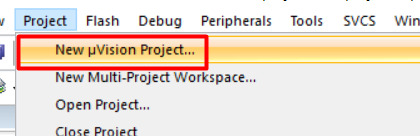
\includegraphics[width=0.8\linewidth]{pics/NewProject.png}
    \caption{New Project.}
    \label{fig:NewProject}
\end{figure}

Choose a place to save it.\\
Then select the device \textit{STM32F107VC}.
\begin{figure}[H]
    \centering
    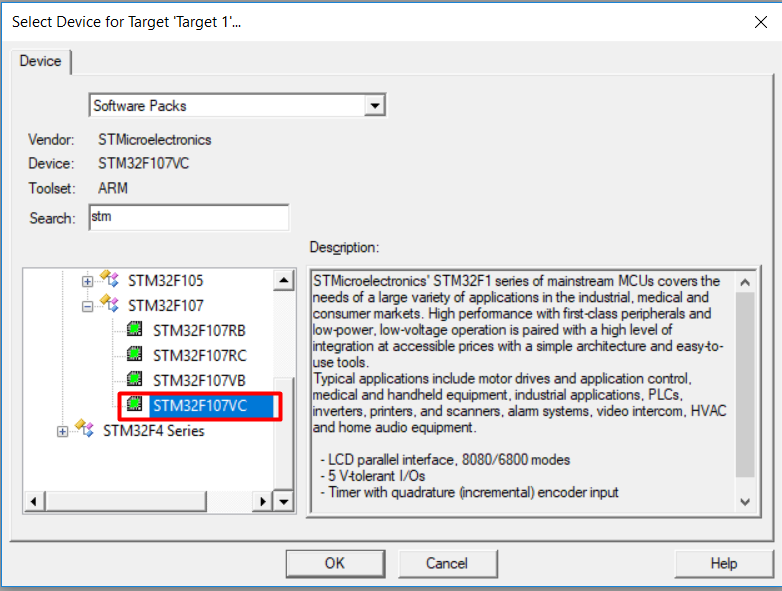
\includegraphics[width=0.8\linewidth]{pics/SelectDevice.png}
    \caption{Select Device.}
    \label{fig:SelectDevice}
\end{figure}

\newpage

The Manage Run-Time Environment should open automatically. If it
does not, open it, and make sure the board variant is \textit{MCBSTM32C}.
It defaults to the E variant.
\begin{figure}[H]
    \centering
    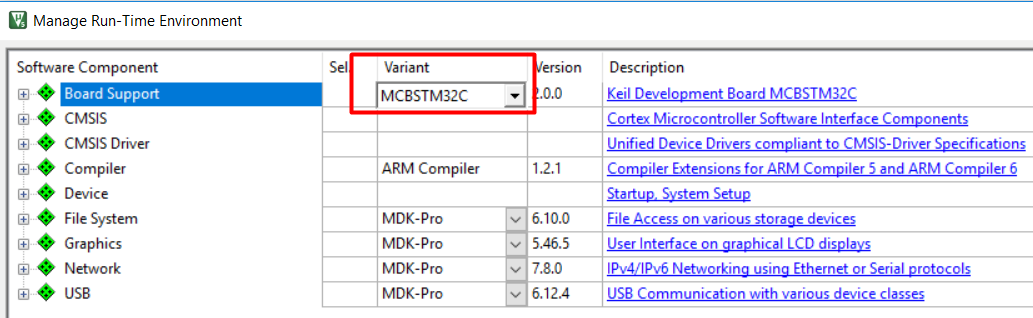
\includegraphics[width=0.8\linewidth]{pics/MRTSetVariant.png}
    \caption{Select Device.}
    \label{fig:SelectDevice}
\end{figure}

Also make sure CMSIS$\to$Core, RTOS$\to$Keil RTX and Device$\to$Startup is selected.
\begin{figure}[H]
    \centering
    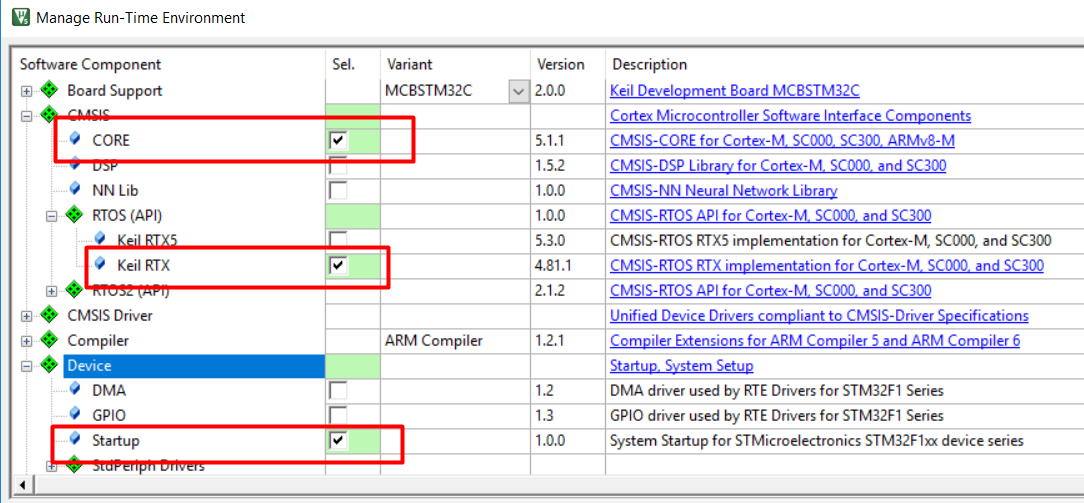
\includegraphics[width=0.8\linewidth]{pics/BasicRuntimeSelection.png}
    \caption{Run time selection.}
    \label{fig:BasicRuntimeSelection}
\end{figure}

Now we want our main .c file, I have called it \textit{tutorial.c}.
In the project pane, expand project, expand the target, then right click the
source group, and select 'Add New Item'. Select a C filetype, and type in the name.
\begin{figure}[H]
    \centering
    \begin{subfigure}[b]{0.45\linewidth}
        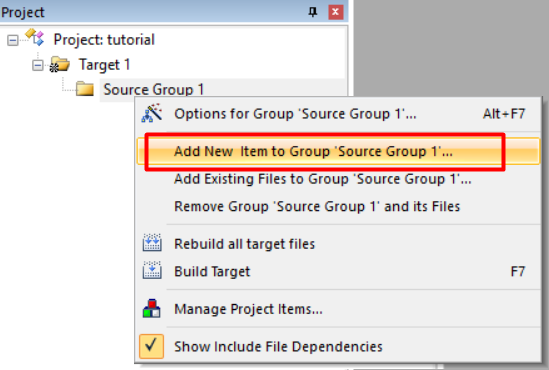
\includegraphics[width=\linewidth]{pics/AddNewFile.png}
        \caption{Add new file.}
    \end{subfigure}
    \begin{subfigure}[b]{0.45\linewidth}
        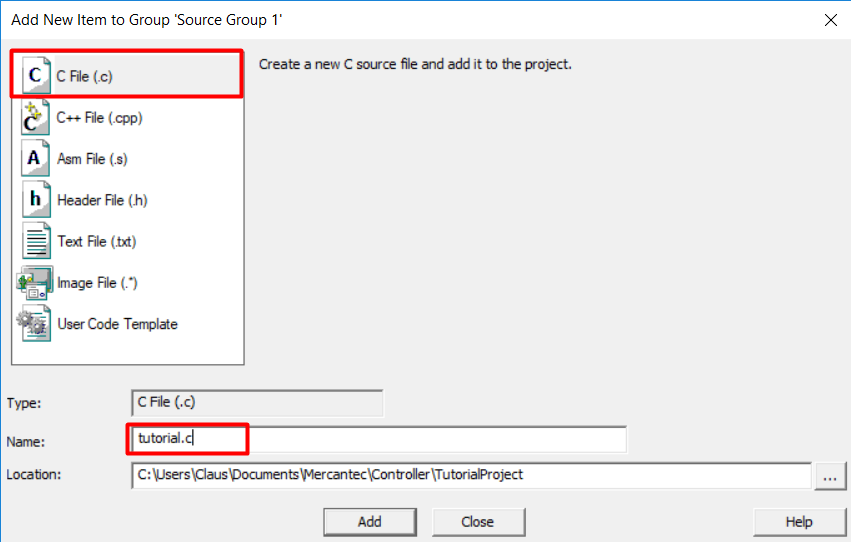
\includegraphics[width=\linewidth]{pics/AddNewFileDialog.png}
        \caption{Type and name.}
    \end{subfigure}
    \label{fig:AddNewFile}
\end{figure}

\newpage

Our project now looks like this, where tutorial.c is empty.
\begin{figure}[H]
    \centering
    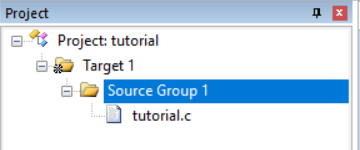
\includegraphics[width=0.5\linewidth]{pics/ProjectStructure1.png}
    \caption{Project Structure.}
    \label{fig:ProjectStructure1}
\end{figure}

We add the most basic code to tutorial.c, and try to compile it.
\begin{figure}[H]
    \centering
    \begin{subfigure}[b]{0.45\linewidth}
        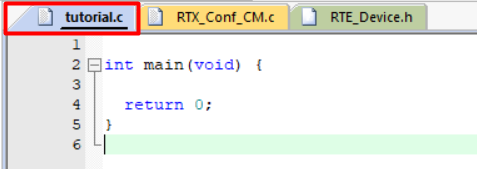
\includegraphics[width=\linewidth]{pics/tutorial_c_basic.png}
        \caption{tutorial.c.}
    \end{subfigure}
    \begin{subfigure}[b]{0.45\linewidth}
        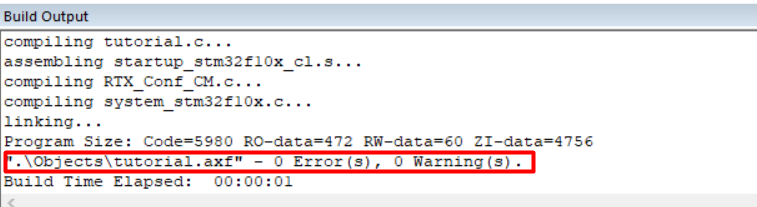
\includegraphics[width=\linewidth]{pics/BasicCompile.png}
        \caption{Compile output.}
    \end{subfigure}
    \label{fig:BasicCode}
\end{figure}

Open Target Options
\begin{figure}[H]
    \centering
    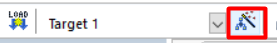
\includegraphics[width=0.5\linewidth]{pics/TargetOptions.png}
    \caption{Target Options.}
    \label{fig:ResetAndRun}
\end{figure}

Open the debug settings, and enable reset and run
\begin{figure}[H]
    \centering
    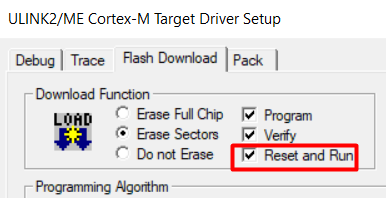
\includegraphics[width=0.5\linewidth]{pics/ResetAndRun.png}
    \caption{Reset and run.}
    \label{fig:ResetAndRun}
\end{figure}

You can load the program on to the chip, though it will do nothing at this point.
\begin{figure}[H]
    \centering
    \begin{subfigure}[b]{0.3\linewidth}
        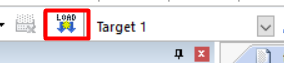
\includegraphics[width=\linewidth]{pics/load.png}
        \caption{Load to device.}
    \end{subfigure}
    \begin{subfigure}[b]{0.6\linewidth}
        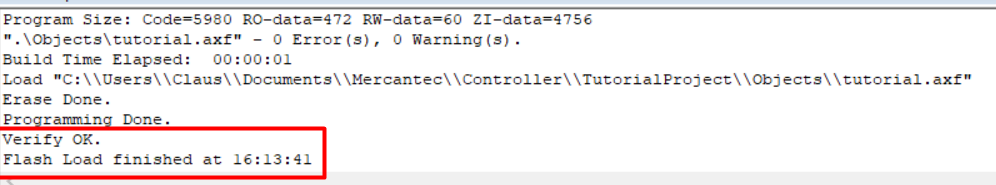
\includegraphics[width=\linewidth]{pics/loadOk.png}
        \caption{Load output.}
    \end{subfigure}
    \label{fig:BasicLoad}
\end{figure}

At this point, the very basic Structure for a project is there, and we're ready
to move on. As someone who's not entirely sure what we're doing, we want debugging output next.

\newpage
\section{Debugging using printf}
First, there's some setup to do.\\
Like before, open the target options. Set the Xtal frequency to 25MHz. Then, also like before,
open the debug settings and set the core clock to 72MHz.
\begin{figure}[h!]
    \centering
    \begin{subfigure}[b]{0.45\linewidth}
        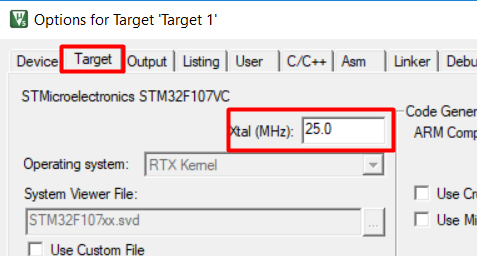
\includegraphics[width=\linewidth]{pics/Xtal.png}
        \caption{Xtal.}
    \end{subfigure}
    \begin{subfigure}[b]{0.45\linewidth}
        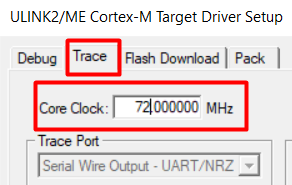
\includegraphics[width=\linewidth]{pics/DebugCoreClock.png}
        \caption{Core clock.}
    \end{subfigure}
    \label{fig:Xtal}
\end{figure}

Open the Run-Time Environment Manager, and make sure \textit{STDERR}, \textit{STDIN}
and \textit{STDOUT} in Compiler$\to$I/O is set to \textit{ITM}.
\begin{figure}[h!]
    \centering
    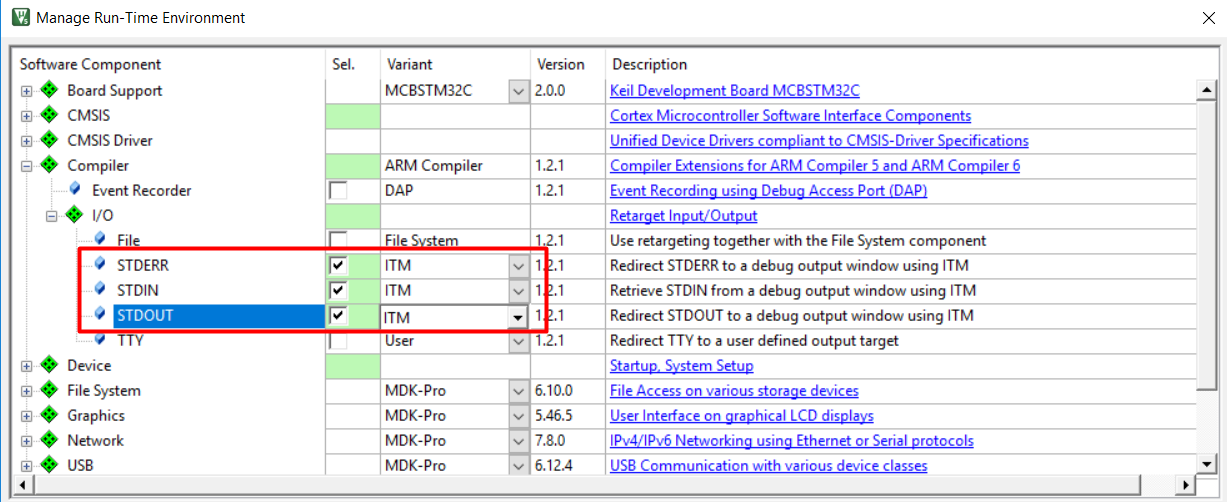
\includegraphics[width=0.8\linewidth]{pics/RuntimeDebug.png}
    \caption{Run time debug settings.}
    \label{fig:Run time debug settings}
\end{figure}

\newpage

In Target Options$\to$Debug$\to$Settings enable Trace, disable timestamps(I found them to generate quite a bit of traffic)
and set the ITM Stimulus Ports.
\begin{figure}[H]
    \centering
    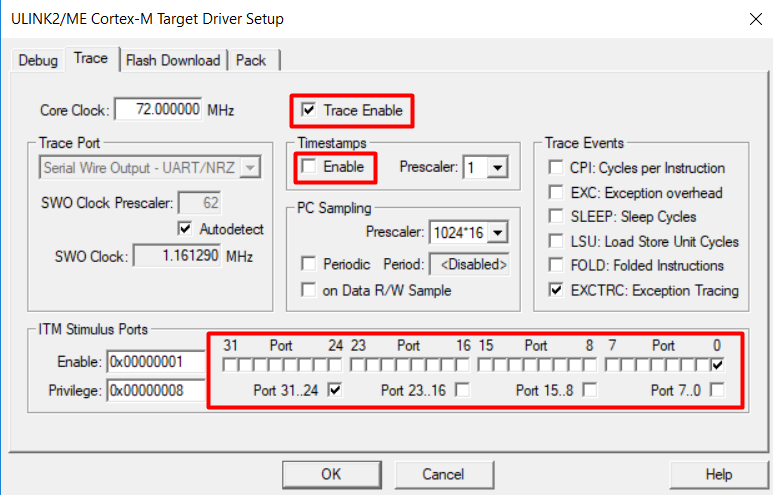
\includegraphics[width=0.8\linewidth]{pics/TraceSetup.png}
    \caption{Trace settings.}
    \label{fig:TraceSettings}
\end{figure}

Apparently printf statements use quite a bit of memory, so we need to increase the stacks size available.
Open the file \textit{CMSIS/RTX\_Conf\_CM.c}, and select the configuration wizard tab.
Here, increase the stacks size.
\begin{figure}[H]
    \centering
    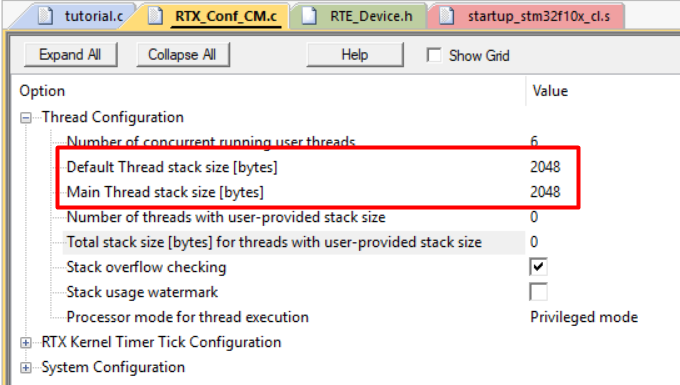
\includegraphics[width=0.8\linewidth]{pics/ThreadStackSize.png}
    \caption{Stacks size.}
    \label{fig:StackSize}
\end{figure}

\newpage

Add a bit more code to \textit{tutorial.c}.\\
We add \textit{stdio.h} to get access to \textit{printf}, and \textit{cmsis\_os.h}
to get access to \textit{osDelay}.
\begin{figure}[H]
    \centering
    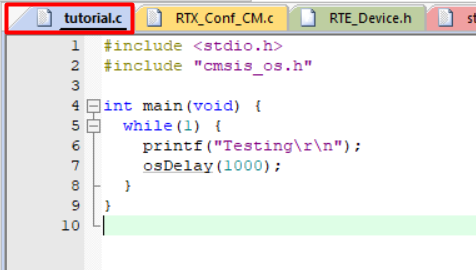
\includegraphics[width=0.8\linewidth]{pics/PrintfMain.png}
    \caption{More code.}
    \label{fig:ModeCode}
\end{figure}

Compile the code, and start the debugger.
\begin{figure}[H]
    \centering
    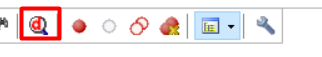
\includegraphics[width=0.5\linewidth]{pics/StartDebugger.png}
    \caption{Start the debugger.}
    \label{fig:StartDebugger}
\end{figure}

\newpage

Open the printf debug viewer.
\begin{figure}[H]
    \centering
    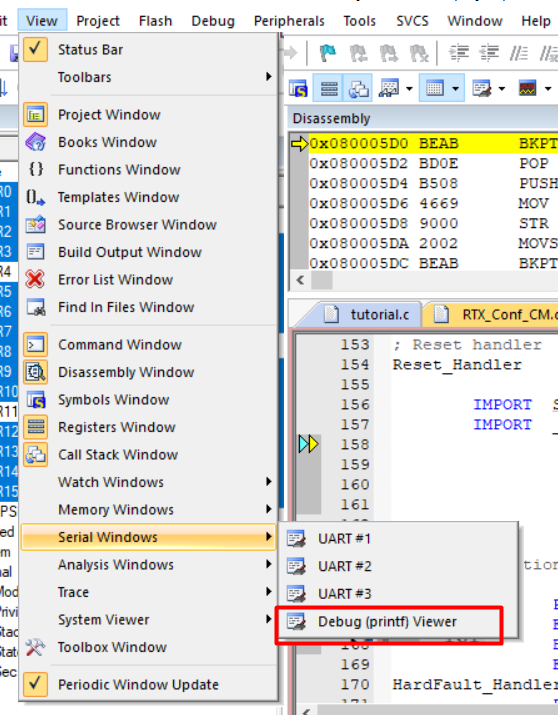
\includegraphics[width=0.8\linewidth]{pics/DebugWindow.png}
    \caption{Debug window.}
    \label{fig:DebugWindow}
\end{figure}

Start the debug session.
\begin{figure}[H]
    \centering
    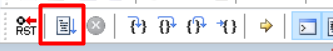
\includegraphics[width=0.5\linewidth]{pics/RunDebugSession.png}
    \caption{Start debug.}
    \label{fig:StartDebugger}
\end{figure}

\newpage

And the output from the printf statement should appear in the debug window.
\begin{figure}[H]
    \centering
    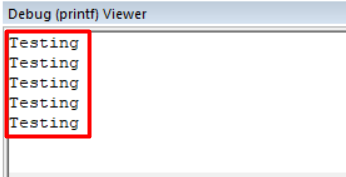
\includegraphics[width=0.5\linewidth]{pics/DebugOutput.png}
    \caption{Debug output.}
    \label{fig:DebugOutput}
\end{figure}

\section{LCD}

\section{I2C \& Accelerometer}

%\begin{lstlisting}
%int main (void) {

%    LED_Initialize();
%    InitDisplay();
%    I2C_Initialize();
    
%    osKernelInitialize();                     
    
%    TID_Led = osThreadCreate(osThread(BlinkLed), NULL);
%    TID_Display = osThreadCreate(osThread(Display),  NULL);
%    TID_I2C = osThreadCreate(osThread(I2CHandler), NULL);

%    osKernelStart(); 

%    while(1);
%}
%\end{lstlisting}


%Hello World!
\end{document}
